\section*{Klasa chessPlus}
Klasa chessPlus powstała jako rozszerzenie klasy Board z biblioteki chess. Naprawia ona kilka problemów związanych z zmianą perspektywy planszy, a także dodaje kilka bardzo ważnych metod enkodujących i dekodujących ruchy oraz plansze.

\section*{Zmiana perspektywy}
Zmiana perspektywy jest bardzo istotną częścią działania opisywanego algorytmu. Dzięki niej model nie musi uczyć się ruchów dla obu graczy, lecz jedynie dla białych figur. Zmiana perspektywy polega na zamianie kolorów oraz obróceniu planszy względem przekątnej. Czyli najpierw obracamy względem osi x, a następnie y. Biblioteka chess posiada w pełni działającą metodę \textit{apply\_mirror()}, która obraca planszę względem osi x, zmieniając jednocześnie kolory figur. Problem pojawia się przy obrocie względem osi y. Bilioteka zawiera generyczną metodę \textit{apply\_transform()} przyjmującą jako argument funkcję transformującą. W naszym przypadku jest to funkcja \textit{flip\_horizontal()}, która wykonuje operacje bitowe na opisujących plansze liczbach 64 bitowych. Mimo powyższych operacji, po wykonaniu obrotu nie działa poprawnie metoda \textit{push()}, która wykonuje ruch na planszy. Problemem są roszady...

\section*{Rozwiązanie problemu z roszadami}
Metoda \textit{push()} zaraz po wywołaniu sprawdza warunki roszady. Jeżeli nie są one spełnione to prawa do roszady zostają wyzerowane. Problem pojawia się w momencie kiedy plansza jest obrócona względem osi y. Autor biblioteki nie uwzględnił takiego obrotu i sztywno napisał warunki sprawdzające pozycje figur. Czego skutkiem są zerowane prawa do roszady. W celu naprawienia tego problemu, została stworzona metoda \textit{better\_clean\_castling\_rights()}, która uwzględnia obrót planszy.

\lstset{style=codeListingStyle}
\begin{lstlisting}[
    language=Python, 
    caption=poprawiony fragment metody clean castling rights,
    inputencoding=utf8
]
white_castling &= (chess.BB_A1 | chess.BB_H1)
black_castling &= (chess.BB_A8 | chess.BB_H8)

if not self.occupied_co[chess.WHITE] & self.kings & ~self.promoted & (chess.BB_D1 if self.changed_perspective else chess.BB_E1):
    white_castling = 0
if not self.occupied_co[chess.BLACK] & self.kings & ~self.promoted & (chess.BB_D8 if self.changed_perspective else chess.BB_E8):
    black_castling = 0

return white_castling | black_castling
\end{lstlisting}

W podobny sposób została naprawiona dalsza część metody \textit{push()} odpowiedzialna za roszady. W pierwszej kolejności została zdmodyfikowana metoda \textit{to\_chess960} tak aby uwzględniała transformacje planszy. Jest ona wywoływana na początku metody \textit{push()} i konwertuje ruch na standard chess960. Zamienia ona ruch w taki sposób, że przestawiając króla na pole obok wieży, zmienna \textit{move.to\_square} wskazywała na wieże. Takie obejście zostało zastosowane, gdyż biblioteka chess nie umożliwia formalnie postawienia swojej figury na zajętym polu przez swoje figury.

\begin{figure}[!h]
\centering
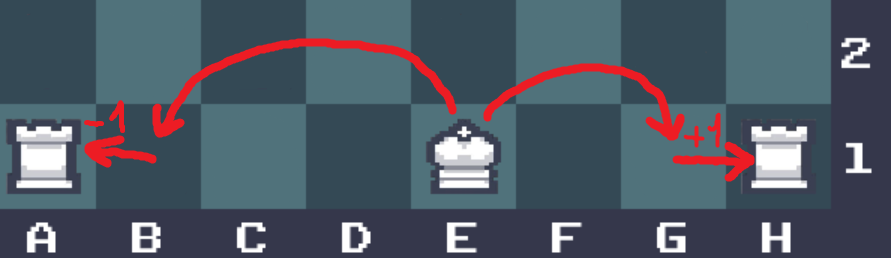
\includegraphics[width=0.8\textwidth]{images/board with castling.png}
\caption{Działanie metody to\_chess960}
\end{figure}

Po powyższych operacjach, metoda \textit{push()} usuwa figury i ustawia je na nowych pozycjach wraz z uwzględnieniem obrotu.

\section*{Dekodowanie planszy}
Dekodowanie planszy polega na stworzeniu 13 binarnych macierzy 8x8, gdzie każda z nich reprezentuje inny typ figury wraz z kolorem. Ostatnia z nich wskazuje na puste pola. Po zakodowaniu planszy, macieże są spłaszczane do jednego wektora o długości 832. 

\section*{Dekodowanie i enkodowanie ruchów}
Rodzai ruchów w szachach jest dokładnie 98. Jeżeli weźmiemy pod uwagę liczbę pól na planszy to jest ich dokładnie 6272. Są one zapisywane podobnie jak plansza, czyli w postaci trój wymiarowej macierzy 8x8x13. Gdzie pierwsze dwa wymiary reprezentują pole gdzie znajduje się figura, a trzeci wymiar reprezentuje indeks ruchu.

Ruchy pionka są najprostszymi ruchami, gdyż ograniczają się tylko do 4 ruchów: ruch do przodu i bicie na skos. Jako nieliczne są obliczane używając różnicy między docelowym, a obecnym polem. (\textit{move.from\_square - move.to\_square}). Zostały one zaprezentowane na poniższym rysunku:
\begin{figure}[!h]
\centering
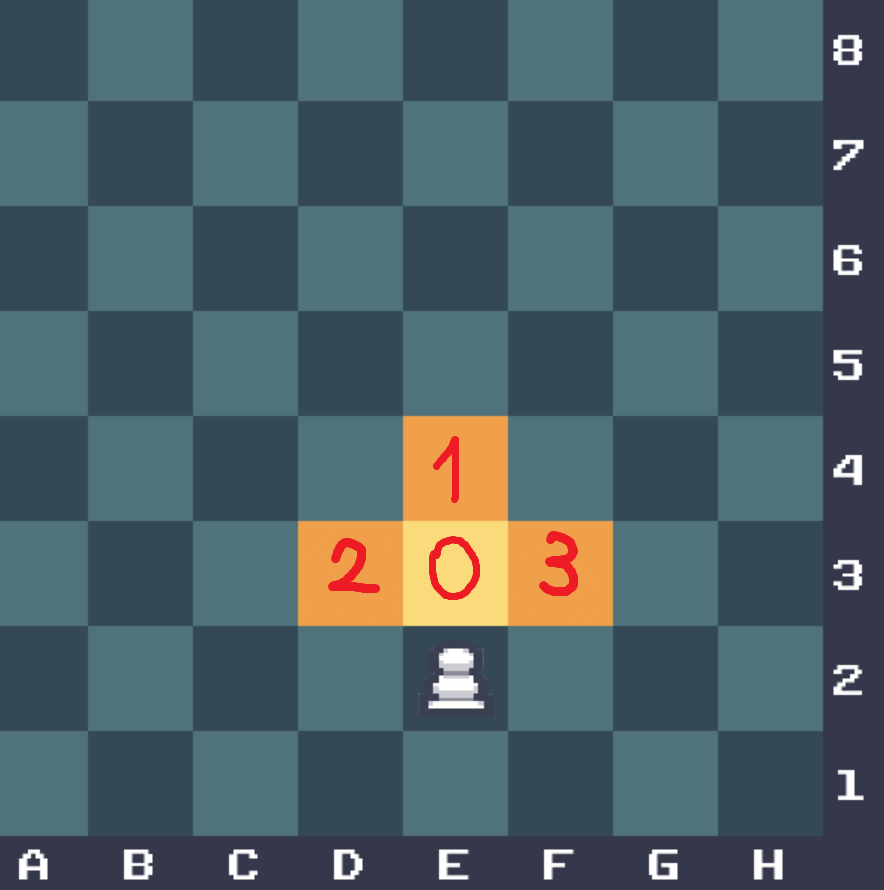
\includegraphics[width=0.4\textwidth]{images/pawn_moves.png}
\caption{Indeksowanie ruchów pionka}
\end{figure}

Ruchy skoczka zostały zaimplementowane tak samo. Zostały one zaprezentowane na poniższym rysunku:

\begin{figure}[!h]
\centering
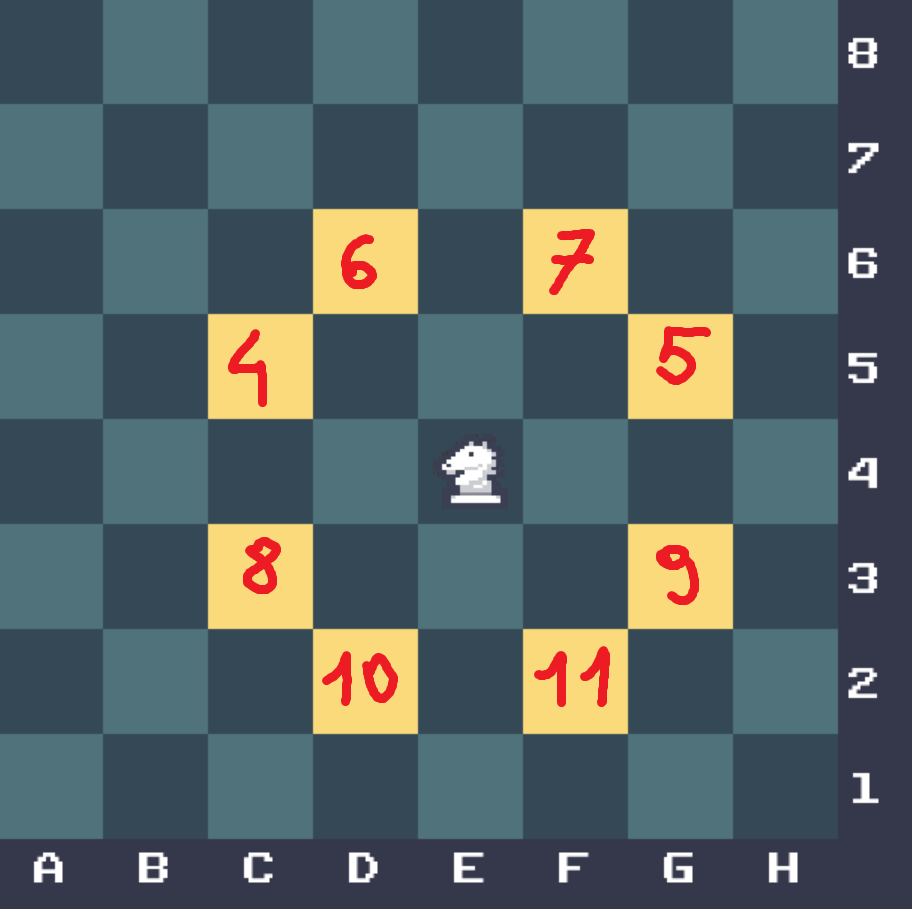
\includegraphics[width=0.4\textwidth]{images/knight_moves.png}
\caption{Indeksowanie ruchów skoczka}
\end{figure}

Indeksowanie ruchów gońca jest podzielone na lewą i prawą stronę. Dodatkowo jest uwzględniany wiersz na który chcemy wykonać ruch. Na przykład jeżeli chcemy wykonać ruch z pola E4 na C6 to jest to ruch w lewą stronę do wiersza 6, co jest reprezentowane przez indeks nr 25. Taki sposób działa niczym winda, gdzie wybieramy na jakie piętro chcemy wjechać. Sposób ten jest efektywny w porównaniu do obliczania różnicy pól, gdyż w najgorszym przypadku potrzebowalibyśmy aż 32 indeksów (4 strony po 8 wierszy), co jest 2 razy więcej niż opisywany sposób.
Indeksowanie ruchów wieży jest identyczne jak gońca, z tą różnicą że zamiast lewej i prawej strony, jest rozróznianie między ruchem pionowym i poziomym.
\begin{figure}[h]
\centering
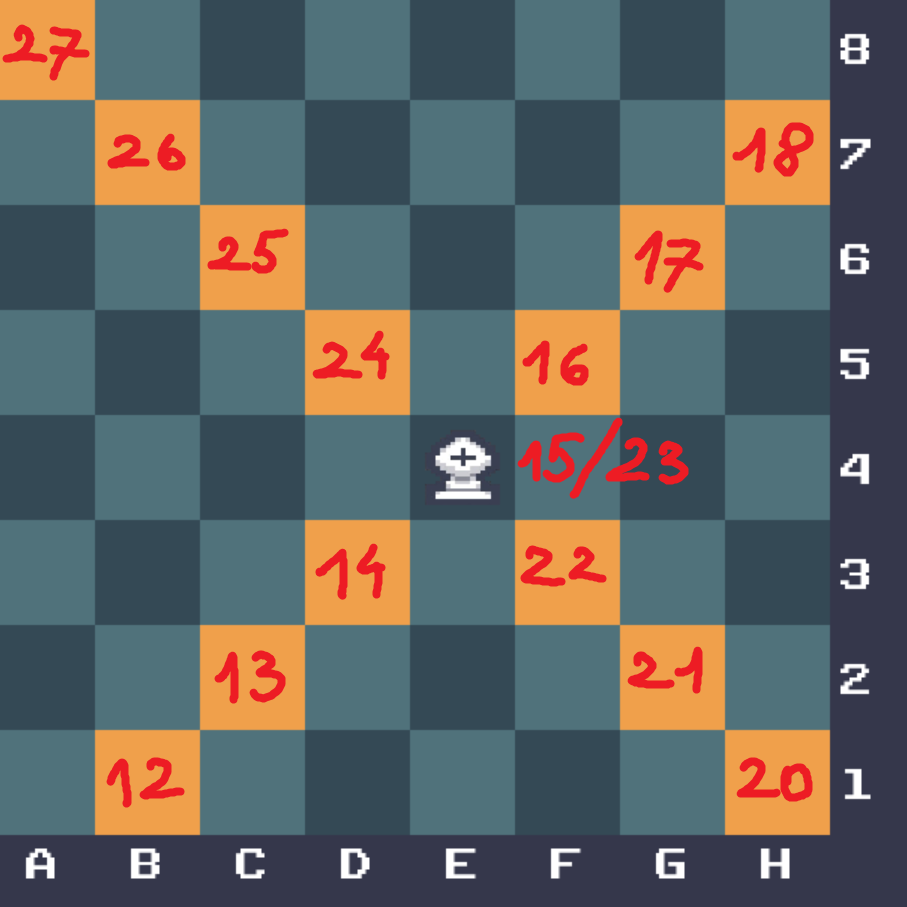
\includegraphics[width=0.4\textwidth]{images/bishop_moves.png}
\hspace{1cm}
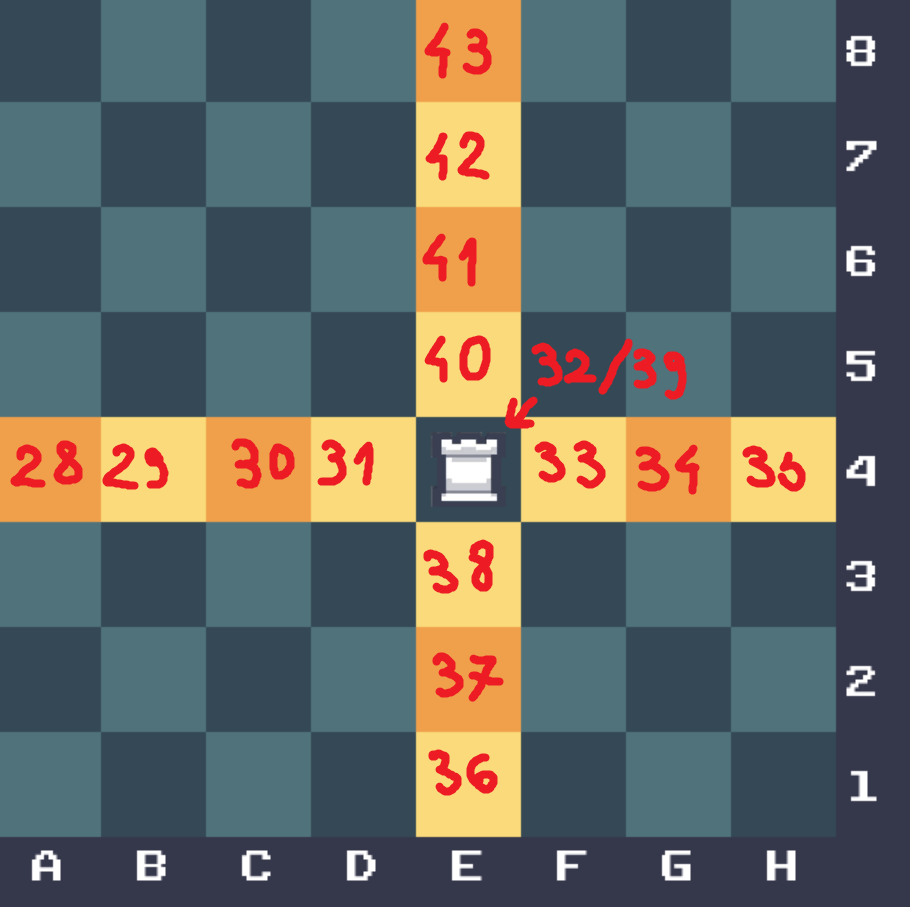
\includegraphics[width=0.4\textwidth]{images/rook_moves.png}
\caption{Indeksowanie ruchów gońca i wieży}
\end{figure}

Indeksowanie ruchów króla działa jak w przypadku pionków oraz skoczka. Natomiast hetman jest połączeniem ruchów gońca i wieży.

\begin{figure}[h]
\centering
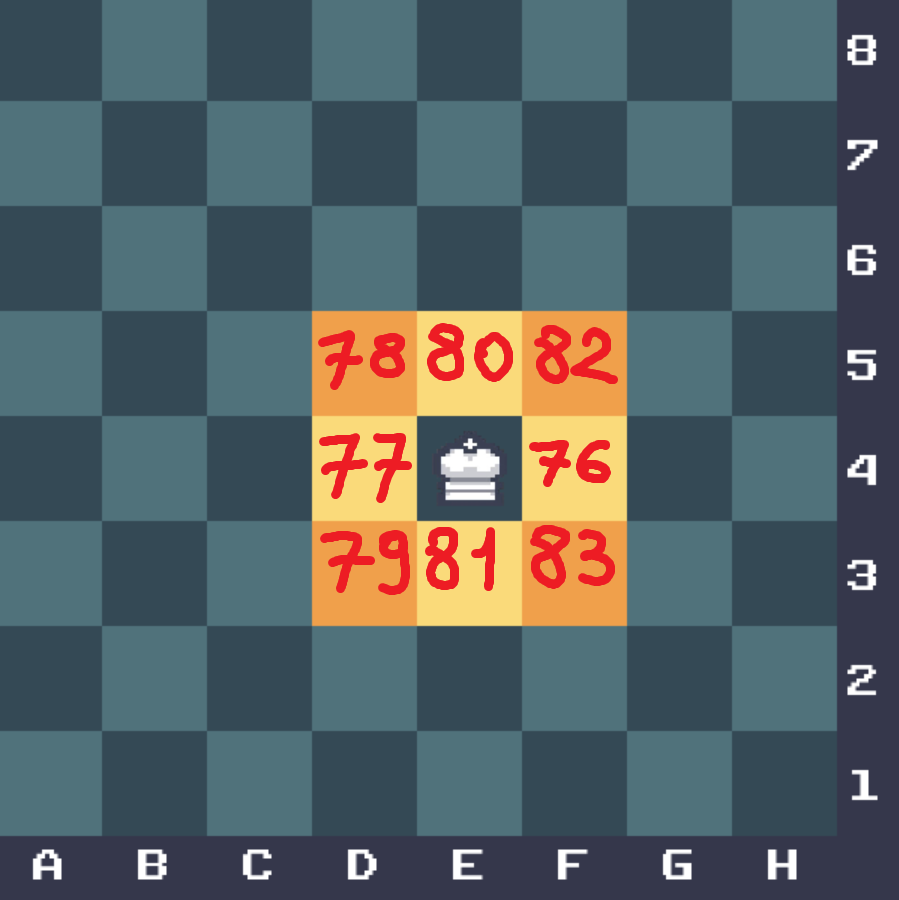
\includegraphics[width=0.4\textwidth]{images/king_moves.png}
\hspace{1cm}
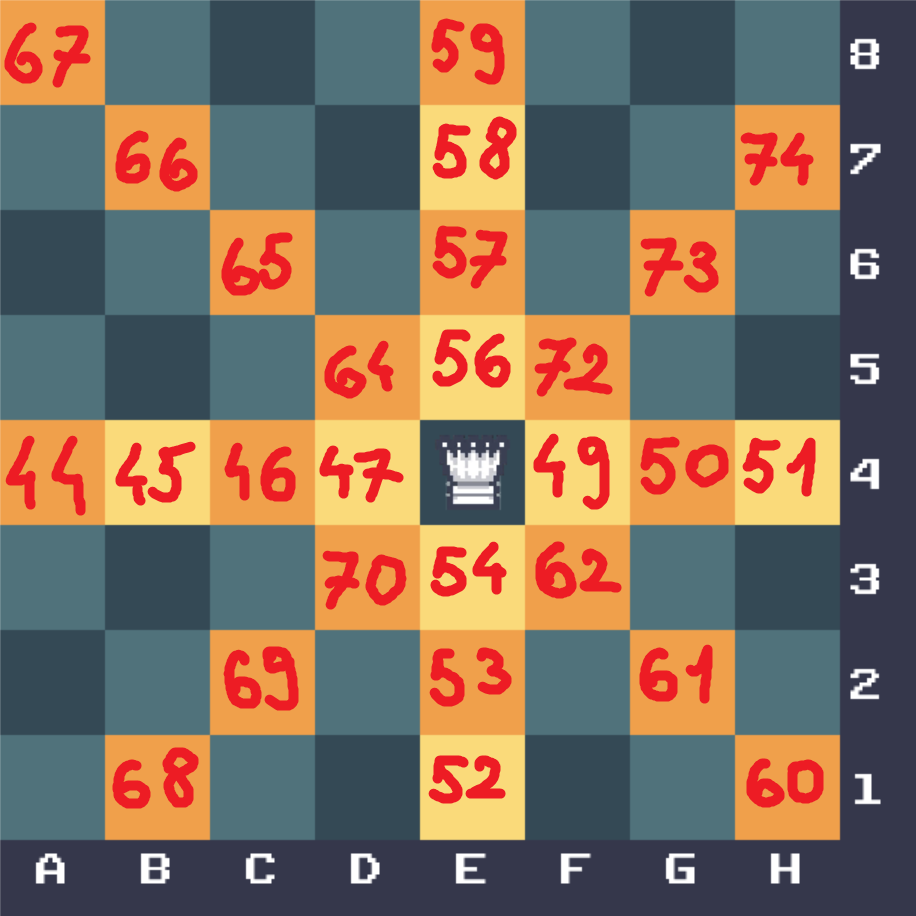
\includegraphics[width=0.4\textwidth]{images/queen_moves.png}
\caption{Indeksowanie ruchów króla i hetmana}
\end{figure}
